% !TEX TS-program = pdflatex
% !TEX encoding = UTF-8 Unicode

\documentclass[12pt]{article} % "article", "book", "report", "letter"
\linespread{1.3}

\usepackage{polski}
\usepackage[utf8]{inputenc} %Win: "cp1250", Linux: "latin2", "utf8"

\usepackage{geometry} % geometria strony
\geometry{a4paper} % "letterpaper", "a5paper"
\geometry{margin=20mm}
% \geometry{landscape} % dla poziomych stron
\usepackage{wrapfig}
\usepackage{graphicx} % dla grafik z uzyciem "\includegraphics"
\usepackage{hyperref}
\title{Instrukcja użytkownika systemu konsultacji}


% Poczatek dokumentu

\begin{document}
\maketitle
\newpage

\section{Opis systemu}
Celem aplikacji jest udostępnianie i zarządzanie konsultacjami prowadzących na
Politechnice Wrocławskiej. Aplikacja dostępna jest pod adresem
\underline{konsultacje.iiar.pwr.wroc.pl}. Zmiany dokonane za pomocą serwisu są
automatycznie umieszczane na stronie
\underline{http://www.iiar.pwr.wroc.pl/iiar/}.


\section{Kurs Obsługi}
\subsection {Strona Główna}
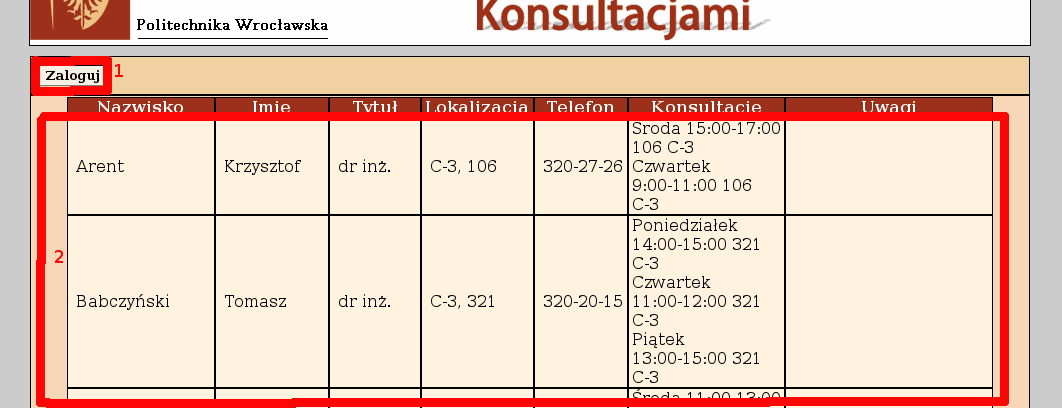
\includegraphics [width=1\textwidth]{instr1.png} 
\\
Na stronie głównej mozemy wywołać ekran logowania \textbf{(1)} oraz przejrzeć
aktualne konsultacje wykładowców \textbf{(2)}.
\subsection {Ekran Logowania}
\begin{wrapfigure}[8]{L}{0.5 \textwidth}

 \begin{center}
 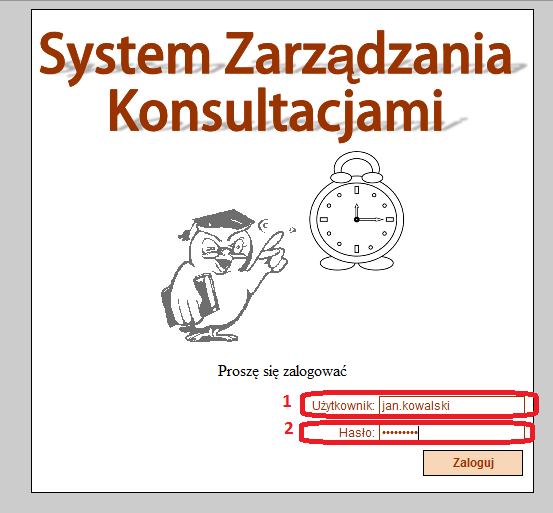
\includegraphics[width=0.4\textwidth]{instr2.png}
 \end{center}


\end{wrapfigure}
W ekranie logowania podajemy nazwę użytkownika \textbf {(1)} oraz hasło \textbf{(2)} - te same których używamy do logowania na poczcie uczelnianej czyli zwykle jest to  \textbf {(1)} imie.nazwisko oraz hasło z poczty. Następnie klikamy zaloguj i przechodzimy do panelu administrowania konsultacjami\\
\newpage


\subsection{Przeglądanie Konsultacji}
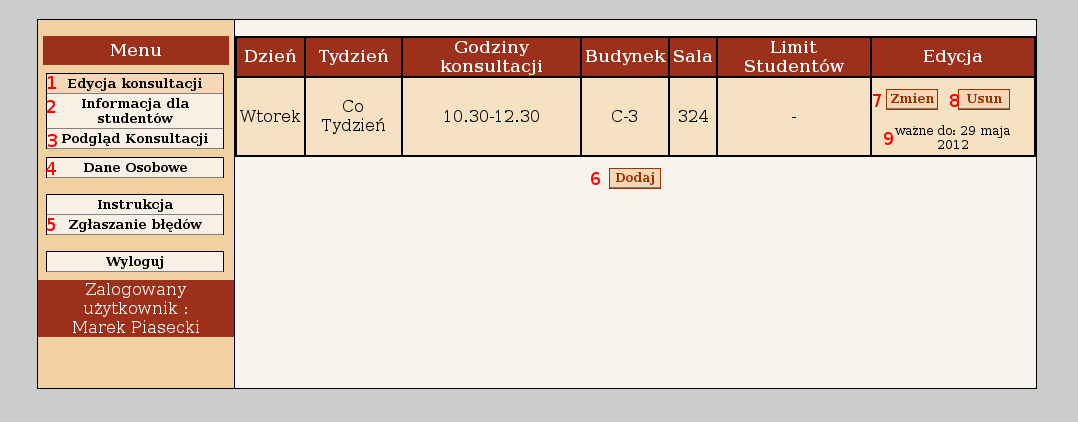
\includegraphics[width=1\textwidth]{instr3.png}
\textbf {(1)}. Ekran przeglądania konsultacji \\
\textbf {(2)}. Dołączenie dodatkowej wiadomości obok informacji z konsultacjami \\
\textbf {(3)}. Podgląd tabeli strony IIAR z konsultacjami(można sprawdzić po
dokonaniu swoich zmian)
\\
\textbf {(4)}. Zmiana danych osobowych \\
\textbf {(5)}. Panel zgłaszania błędów \\
\textbf {(6)}. Przycisk dodawania konsultacji\\
\textbf {(7)}. Przejście do zmiany wybranej konsultacji\\
\textbf {(8)}. Usunięcie wybranej konsultacji\\
\textbf {(9)}. Termin ważności konsultacji - gdy minie wyświetlany jest na
czerwono\\


\subsection{Informacja Dodatkowa}
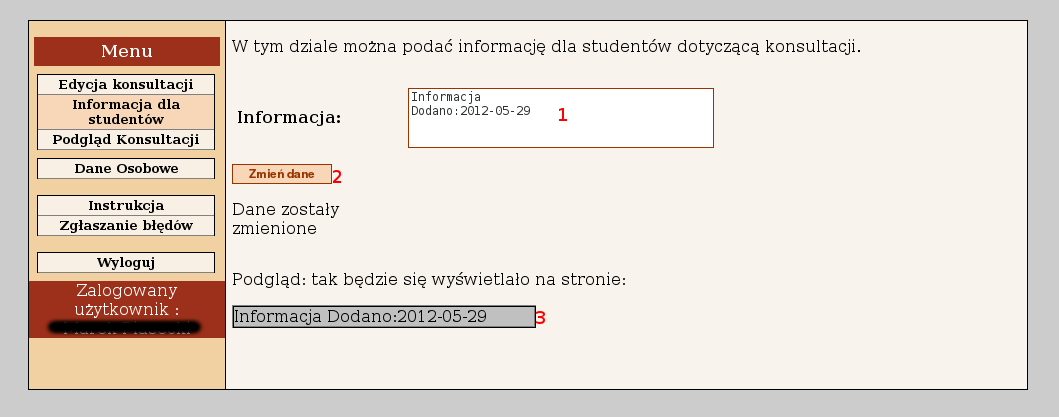
\includegraphics[width=0.8\textwidth]{instr4.png}\\
\textbf {(1)}. Pole edycji wyświetlanej wiadomości\\
\textbf {(2)}. Przycisk do zatwiedzenia zmiany wiadomości\\
\textbf {(3)}. Podgląd informacji wyświetlanej na stronie IIAR


\subsection{Dane Osobowe}
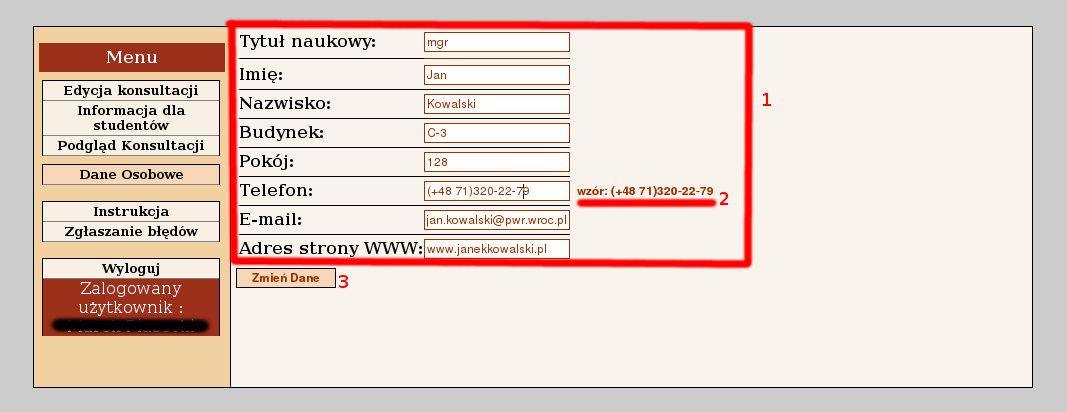
\includegraphics[width=1\textwidth]{instr5.png}\\
\textbf {(1)}. Pola w których można zmieniać dane. Po naciśnięciu na dane pole
po prawej stronie pokazuje się podpowiedź na temat formatu w jakim należy
wprowadzić dane\textbf {(2)}\\
\textbf {(3)}. Przycisk do zatwiedzenia zmiany wiadomości po jego naciśnięciu
pojawi się napis potwierdzający zmianę danych\\


\subsection{Dodawanie Konsultacji}
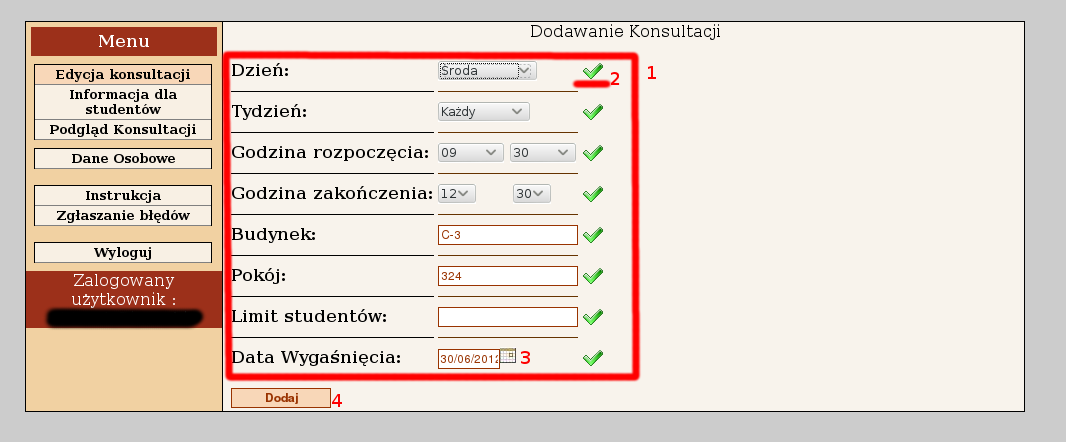
\includegraphics[width=1\textwidth]{instr6.png}\\
\textbf {(1)}. Pola wyboru danych dotyczących konsultacji\\
\textbf {(2)}. Ikonka pojawia się, gdy poprawnie wprowadzono dane. W przeciwnym
wypadku pojawia się informacja
\\
\textbf {(3)}. Po kliknięciu na pole data wygaśnięcia wyświetla się kalendarz z możliwością wyboru daty \\
\textbf {(4)}. Przycisk dodaj pozostaje nieaktywny dopóki wszystkie pola nie są poprawnie uzupełnione\\

\subsection{Edycja Konsultacji}
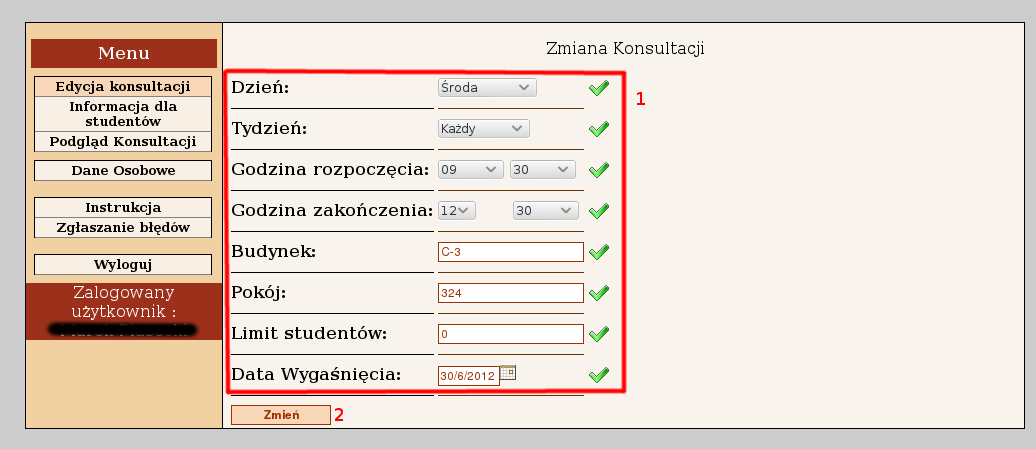
\includegraphics[width=1\textwidth]{instr7.png}\\
\textbf {(1)}. Pola wyboru danych dotyczących konsultacji. Na początku wszystkie
są uzupełnione danymi które aktualnie ma konsultacja którą chcemy edytować.
Znaczniki obok informują o tym, czy dana jest poprawna.\\
\textbf {(2)}.Przycisk Zmień jest aktywny na początku i jak długo wszystkie pola
pozostają poprawnie wypełnione taki pozostaje \\

\subsection{Dodawanie błędów}
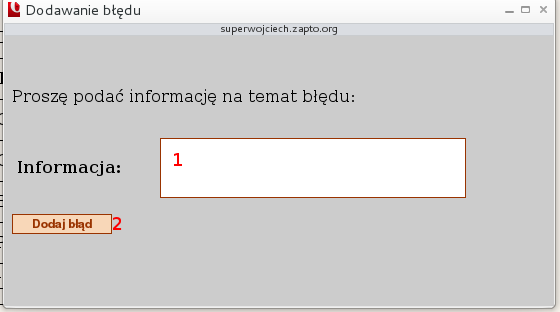
\includegraphics[width=1\textwidth]{instr8.png}\\
\textbf {(1)}. Pole edycji, w którym możemy napisać na czym polega znaleziony
błąd\\
\textbf {(2)}.Przycisk Dodaj błąd zapisuje informację na serwerze. \\

Razem z informacją o błędzie zapisywana jest data zgłoszenia, nazwa użytkownika,
który zgłosił błąd oraz miejsce, w którym błąd nastąpił.

\end{document}